%! Author = goessmann
%! Date = 03.12.25

% Preamble
\documentclass{standalone}
\usepackage{tikz}
\usetikzlibrary{matrix}
\usepackage{xcolor}
\begin{document}

% All the code below must be kept together within the tikzpicture environment
    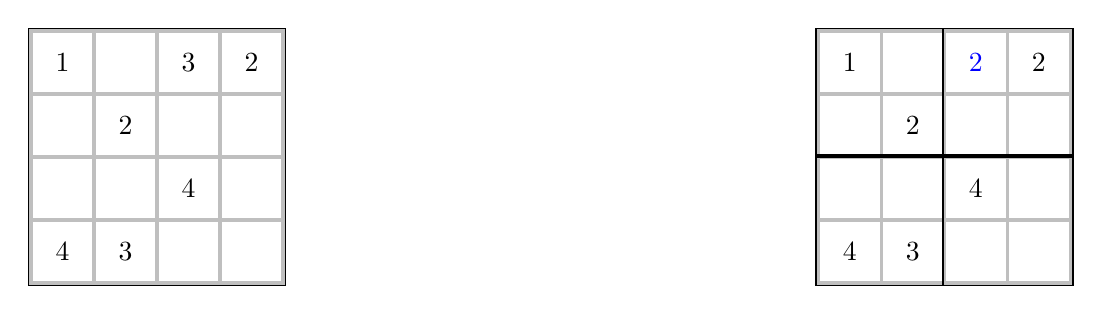
\begin{tikzpicture}[
        sudokucell/.style={
            minimum size=0.8cm, % Adjust cell size here
            draw=gray!50, % Light gray lines for internal grid
            anchor=center
        },
        sudokumatrix/.style={
            matrix of nodes,
            nodes=sudokucell,
            inner sep=0pt,
            row sep=-\pgflinewidth, % Remove space between cells
            column sep=-\pgflinewidth,
            % General border
            draw=black,
            very thick,
        }
    ]

% Draw the Sudoku grid and fill numbers
        \matrix[sudokumatrix] (M) at (0,0) {
            1 & \ & 3 & 2 \\
            \ & 2 & \  & \  \\
            \ & \ & 4 & \ \\
            4 & 3 &  \ & \  \\
        };

        \matrix[sudokumatrix] (M) at (10,0) {
            1 & \ & \textcolor{blue}{2} & 2 \\
            \ & 2 & \  & \  \\
            \ & \ & 4 & \ \\
            4 & 3 &  \ & \  \\
        };
\draw[thick]
  ([yshift=12pt,xshift=-1pt]M-1-2.east) -- ([yshift=-12pt,xshift=-1pt]M-4-2.east);

% Horizontal block separator (between row 2 and 3)
\draw[very thick]
  ([xshift=-12pt,yshift=1pt]M-2-1.south) -- ([xshift=12pt,yshift=1pt]M-2-4.south);
% Vertical middle line: Go from the top edge of the whole matrix (M.north)
% at the X-coordinate of the divider between cells (1,2) and (1,3)

    \end{tikzpicture}

\end{document}